In this chapter we briefly introduce the major principles of
gravitational wave astronomy.  We start in
section~\ref{sec:general_relativity} with a review of general
relativity, starting from the relevant mathematics.  In
section~\ref{sec:gravitational_radiation} we show how general
relativity predicts the existence of gravitational radiation and
discuss some of the properties of this radiation.  Then in
section~\ref{sec:effects_of_waves} we show how gravitational radiation
affects freely-falling particles.  This will motivate the design of
the LIGO experiment to search for gravitational waves, an overview 
which is presented in the next chapter.  We then move to the
generation of gravitational waves and discuss two approaches, analytic
and numerical, for modeling the waves produced by the inspiral and
eventual merger of pairs of neutron stars and/or black holes.



section~\ref{sec:ligo_detectors}.

\section{General Relativity}
\label{sec:general_relativity}

We start with an overview of differential geometry and build to
Einstein's equations.  This is of necessity very brief, readers are
referred to the textbooks by Misner, Thorne and Wheeler~\cite{MTW} and
Carroll~\cite{carrollTextbook} for more complete treatments.

\subsection{Elements of differential geometry}

An $n$-dimensional ($C^\infty$) manifold $\mathcal{M}$ is a set of
points plus an \emph{atlas}, a set of \emph{charts} $\{\phi_i\}$ which
are invertible maps from open subsets of $\mathcal{M}$ to open subsets
of $\mathcal{R}^n$ such that


\begin{itemize}
\item For all points $p \in \mathcal{M}$ there exists an $\phi_i$ 
such that $p$ is in the domain of $\phi_i$.
\item The composition $\phi_i \circ \phi_j^{-1}$ on the 
intersections of the domains of $\phi_i$ and $\phi_j$ is a
($C^\infty$) function from $\mathcal{R}^n \to \mathcal{R}^n$.
\end{itemize}

Two natural structures on a manifold are curves, maps from
$\mathcal{R}\to\mathcal{M}$, and scalar functions,  maps from
$\mathcal{M}\to\mathcal{R}$.  Compositing a function $f$ with a curve
$\gamma(\lambda)$ gives a map from $\mathcal{R} \rightarrow
\mathcal{R}$ which may be differentiated in the usual way at a point
$p$.

\iffalse
\begin{equation*}
\frac{d}{d \lambda} fi \big|_p = 
  \frac{d}{d\lambda} (f \circ \gamma) \big|_p
\end{equation*}


Expanding this in terms of a chart whose domain includes $p$ and then
applying the chain rule
 
\begin{align*}
\frac{d}{d \lambda} fi \big|_p &= 
 \frac{d}{d\lambda} ( (f \circ \phi^{-1}) \circ (\phi \circ
\lambda) ) \\
&= \frac{d(\phi^{-1} \circ \gamma)^\mu}{d\lambda} 
\frac{\partial (f \circ \phi^{-1}) }{\partial x^\mu} \big|_p \\
&= \frac{dx^\mu}{d\lambda} \partial_\mu f \big|_p
\end{align*}

where $x^\mu$ are the coordinates on $\mathcal{R}^n$.  Finally, since
the function $f$ is arbitrary we can define

\begin{equation}
\label{eq:tangent_vector}
\frac{d}{d\lambda} = \frac{dx^\mu}{d\lambda} \partial_\mu
\end{equation}
\fi

Geometrically, taking the derivative gives the tangent vector to the
curve at the point $p$.  It is possible to associate the set of such
vectors with the set of directional derivatives, taking the partial
derivatives along the coordinates as the basis.  Henceforth this basis
will be denoted both $\partial_\mu$ and $\vec{e}_\mu$.

Note that the tangent to a curve is defined at the point $p$.  Each
point in the manifold possesses its own space of tangent vectors.
These spaces are distinct, which will be important in what follows.

We next define \emph{one-forms} as linear maps from vectors to
$\mathcal{R}$.  The set of one-forms at a point can be shown to form a
vector space, a natural basis for which can be obtained by requiring

\begin{equation*}
\vec{e}_\mu \tilde{\omega}^\nu = \delta_\mu^\nu
\end{equation*}

The components of an arbitrary form $\omega$ in this basis may be
found by applying the form to the basis vectors.

\iffalse
\begin{align*}
\omega(\vec{e}_\nu)
&= \tilde{\omega}^\mu \omega_\mu (\vec{e}_\nu) \\
&= \omega_\mu \tilde{\omega}^\mu (\vec{e}_\nu) \\
&= \omega_\mu \delta^\nu_\mu \\
&= \omega_\nu\\
\end{align*}
\fi

We can then build up arbitrary ${m \choose n}$ tensors as linear maps
from tensor products of $m$ vectors and $n$ one-forms to
$\mathcal{R}$.  The components of a tensor $T$ in some coordinates may
found by applying it to combinations of the basis vectors and 1-forms.


Finally, a ${m \choose n}$ tensor field is a map that associates to
each point $p$ in $\mathcal{M}$ an element in the space of  ${m
\choose n}$ tensors at $p$.

\subsection{The metric tensor}

A particularly important tensor in general relativity is the
\emph{metric}, a ${2 \choose 0}$ tensor that is symmetric ($g_{\mu\nu}
= g_{\nu\mu})$ and non-degenerate (the determinant of $g$ taken as a
matrix $|g_{\mu\nu}| \neq 0$.  The latter feature makes it possible to
define the inverse metric $g^{\mu\nu}$ as

\begin{equation*}
g^{\mu_\rho} g_{\rho_\nu} = \delta^\mu_\nu
\end{equation*}

Given a vector $x^\mu$ the object $g_{\mu\nu} x^\mu$ maps another
vector to a real number, and is therefore a one-form.  The metric
therefore maps between the space of one-forms and the space of vectors
at each point.  Most importantly, the metric defines a notion of
distance on the manifold.  Infinitesimally

\begin{equation}
ds^2 = g_{\mu\nu} dx^\mu dx^\nu
\end{equation}

In special relativity, in Cartesian coordinates, the metric has
components $(-1,1,1,1)$ along the diagonal, all other components are
zero.   The metric will be denoted $\eta$ and called the \emph{flat
space metric}.

\subsection{Covariant derivatives}

Since vectors are only defined at a point we need additional structure
to define derivatives of vector fields, as there is no natural way to
compare vectors that live in different spaces.  We seek an operator
$\nabla$ with the following properties

\begin{itemize}
\item Maps ${m \choose n}$ tensors to ${m \choose {n+1}}$ tensors.
This is so we may consider the directional derivative of a tensor $T$
along a vector $x$ as $x^\mu \nabla_\mu T$.
\item Reduces to partial differentiation when applies to a scalar
field.
\item Linear.
\item Satisfies the Leibniz rule, $\nabla(a b) = a\nabla b + b \nabla a$.
\end{itemize}

Such an operator applied to a vector field gives

\begin{equation*}
\nabla_\mu (x^\nu \vec{e}_\mu)
= (\partial x^\nu) \vec{e}_\mu + x^\nu (\nabla_\nu \vec{e}_\mu)
\end{equation*}

In a flat space in Cartesian coordinates the basis vectors do not
change and so the last term is zero.  But in a curved space, or even
flat space in non-Cartesian coordinates, they may.  However, the new
vector must be expressible as a linear combination of the original
basis vectors  The components are called \emph{connection
coefficients} and are denoted as $\Gamma^\rho_{\nu\mu}$ so

\begin{align}
\label{eq:covariant_derivative}
\nabla_\mu (x^\nu \vec{e}_\mu) &= 
(\partial x^\nu) \vec{e}_\mu + 
x^\nu \Gamma^\rho_{\nu\mu} \vec{e}_\rho \\
&= (\partial x^\nu + x^\rho \Gamma^\nu_{\mu\rho}) \vec{e}_\nu \\
\nabla_\mu x^\nu &= \partial x^\nu + x^\rho \Gamma^\nu_{\mu\rho}
\end{align}

In general relativity the connection is usually assumed to be
\emph{torsion-free}, that is

\begin{equation}
\label{eq:torsion}
 \Gamma^\nu_{\mu\rho} =  \Gamma^\nu_{\rho\mu}
\end{equation}

which thus far has been borne out by experiment.  However, it is
possible to construct theories where this condition does not hold.

By considering the covariant derivative of a scalar constructed from a
one-form acting on a vector, $\nabla (x^\nu \omega_nu)$, it can be shown
that

\begin{equation*}
\nabla_\mu \omega_\nu = \partial_\mu \omega_\nu - 
\Gamma^\rho_{\mu\nu} \omega_\rho
\end{equation*}

The covariant derivative of a ${m \choose n}$ tensor generalizes this
and has a partial derivative term, $m$ positive therms in $\Gamma$ and
$n$ negative terms in $\Gamma$.

\subsection{Parallel Transport}
\label{ssec:parallel}

Covariant differentiation provides a way to ``move a vector without
changing it.''  We can \emph{parallel transport} a vector $v^\mu$
infinitesimally along a curve whose tangent vector is $u^\nu$ by
requiring

\begin{equation*}
u^\nu \nabla_\nu v^\mu = 0
\end{equation*}

As an example of such transport, consider an arrow on the equator of
the Earth pointing towards the north pole.  This arrow can be carried
halfway around the equator without rotating it, so it ends up on the
other side of the globe, still pointing north.  If the vector is then
parallel transported northward to the pole and then continued until it
returns to its starting point it will return pointing south.  Although
the vector was never rotated locally it has returned rotated.  This is
an indication that the underlying space is curved.

Of particular interest is the case where a vector is
parallel-transported along itself

\begin{equation*}
0 = v^\mu \nabla_\mu v^\nu 
= v^\mu (\partial_\mu v^\nu + \Gamma^\nu_{\mu\rho} v^\rho)
\end{equation*}

Now consider a curve $x(\lambda)$ such that $v$ is the tangent to this
curve, $v^\mu = d x^\mu/d\lambda$, then

\begin{align}
\label{eq:geodesic}
\frac{d x^\mu}{d\lambda}
  \frac{\partial }{\partial x^\mu}
  \frac{d x^\nu}{d\lambda}  
+ \Gamma^\nu_{\mu\rho} 
\frac{d x^\mu}{d\lambda}
\frac{d x^\rho}{d\lambda} &= 0 \nonumber \\
\frac{d^2 x^\nu}{d\lambda^2}
+ \Gamma^\nu_{\mu\rho} 
\frac{d x^\mu}{d\lambda}
\frac{d x^\rho}{d\lambda} &= 0 \nonumber \\
\end{align}

This is the \emph{geodesic equation}, solutions to which are
\emph{geodesics}.  The same equation can be derived by extremizing
the path length, $\sqrt{g_{\mu\nu} dx^\mu dx^\nu}$.

In general relativity test masses acting under the influence of
gravity and no other forces follow geodesics.  

\subsection{The Christoffel Symbols}

If we now require that scalars do not change under parallel transport
we have, for arbitrary vectors fields $u^\alpha, v^\beta$ and $x^\mu$

\begin{align*}
0 &= x^\mu \nabla_\mu (g_{\alpha\beta} u^\alpha v^\beta) \\
&= x^\mu (\nabla_\mu g_{\alpha\beta}) u^\alpha v^\beta
+ g^{\alpha\beta} (x^\mu \nabla_\mu u^\alpha) v^\beta
+ g^{\alpha\beta} u^\alpha (x^\mu \nabla_\mu v^\beta)
\end{align*}

We can now specialize such that $u^\alpha, v^\beta$ are constant
and so the last two terms vanish, which implies the  \emph{metric
compatibility} condition:

\begin{equation}
\label{eq:metric_compatibility}
\nabla_\mu g_{\alpha\beta} = 0
\end{equation}

Equations~\ref{eq:metric_compatibility} and~\ref{eq:torsion} together
fix the connection coefficients in terms of the metric:

\begin{equation}
\Gamma^{\rho}{\mu\nu}
= \frac{1}{2} g^{\rho\sigma}\left[
\partial_\nu g_{\mu\sigma}
+ \partial_\mu g_{\nu\sigma}
- \partial_\sigma g_{\mu\nu}
\right]
\end{equation}


Combining this with the previous section we see that the motion of a
particle is completely specified once we know the metric.

\subsection{The Riemann Tensor}

We now generalize the example given in section~\ref{ssec:parallel}, and
ask how a vector $A^\mu$ changes as it is parallel-transported around
an infinitesimal parallelogram with sides defined by the vectors
$B^\mu$ and $C^\nu$.  Recalling that vectors and directional
derivatives are the same thing, it can be shown that this is
equivalent to asking how covariant derivatives fail to commute.  The
result must be linear in the vectors and so we may write

\begin{equation}
\label{eq:riemann_def}
\left[\nabla_\mu \nabla_\nu - \nabla_\nu \nabla_\mu\right] A^\rho
= R^\rho_{\sigma\mu\nu} A^\sigma
\end{equation}

which defines the \emph{Riemann tensor} $R^\rho_{\sigma\mu\nu}$.  A
number of properties follow from this definition (which are either
obvious or may be proven by substituting the definition of the
covariant derivative, eqn.~\ref{eq:covariant_derivative}).

First, the symmetry properties

\begin{equation}
\label{eq:symmetries}
R_{\rho\sigma\mu\nu}
= -R_{\sigma\rho\mu\nu}
= -R_{\rho\sigma\nu\mu}
= R_{\mu\nu\rho\sigma}
\end{equation}

which in turn imply

\begin{align}
R^\rho_{[\sigma\mu\nu]} = 0
\end{align}

Second, the Bianchi identity,

\begin{equation}
\label{eq:bianchi}
R_{\rho\sigma\mu\nu;\alpha}
+R_{\rho\sigma\nu\alpha;\mu}
+R_{\rho\sigma\alpha\mu;\nu} = 0
\end{equation}

We may now generalize equation~\ref{eq:riemann_def} and ask how an
arbitrary tensor changes after being parallel-transported 
around a loop.  It can be shown that

\begin{equation}
\label{eq:higher_order_riemann}
\left[\nabla_\mu \nabla_\nu - \nabla_\nu \nabla_\mu\right] 
B^{\rho_1 \rho_2 \ldots \rho_n}
= - R^{\rho_1}_{\sigma \mu\nu} B^{\sigma \rho_2 \ldots \rho_n}
- R^{\rho_2}_{\sigma \mu\nu} B^{\rho_1 \sigma \ldots \rho_n}
- \ldots -
- R^{\rho_n}_{\sigma \mu\nu} B^{\rho_1 \rho_2 \ldots \sigma }
\end{equation}

which may be proved by expanding

\begin{equation*}
\left[\nabla_\mu \nabla_\nu - \nabla_\nu \nabla_\mu\right] 
(\vec{e}_\rho \otimes \vec{e}_\sigma)
\end{equation*}

and then proceeding by induction.  

The symmetries of the Riemann tensor imply that there is, up to sign,
only one non-trivial contraction

\begin{equation}
R_{\mu\nu} = R^\sigma_{\mu\sigma\nu}
\end{equation}

which defines the \emph{Ricci tensor}.  This may be contracted again

\begin{equation}
R = R^\mu_\mu
\end{equation}

to obtain the \emph{Ricci scalar}.

Contracting the Bianchi identity twice gives

\begin{equation*}
g^{\sigma\nu}
\left(\nabla_\alpha R_{\sigma\nu}
+ \nabla^\rho R_{\rho\sigma\nu\alpha}
+ \nabla_\nu R^\mu_{\sigma\alpha\mu}\right) = 0
\end{equation*}

Using the symmetries of the Riemann tensor (eqn.~\ref{eq:symmetries})
this can be written

\begin{equation*}
\nabla_\alpha R
- \nabla^\rho R_{\rho\alpha}
- \nabla^\sigma R_{\sigma\alpha} = 0
\end{equation*}

Relabeling the dummy indices and using metric compatibility gives

\begin{equation*}
\nabla^\rho \left(g_{\rho\alpha} R - 2 R_{\rho\alpha} \right) = 0
\end{equation*}

This motivates the definition of the \emph{Einstein Tensor} as

\begin{equation}
\label{eq:einstein_tensor}
G_{\mu\nu} = R_{\mu\nu} - \frac{1}{2} g_{\mu\nu} R
\end{equation}

the previous result implies this is divergentless

\begin{equation*}
\nabla^\nu G_{\mu\nu} = 0
\end{equation*}

Note that $G$ is also symmetric, $G_{\mu\nu} = G_{\nu\mu}$.

We now relate this to physics by noting that the matter and energy
content of a region is described by the stress-energy tensor
$T_{\mu\nu}$ where each component is ``the flow of $\mu$ momentum in the
$\nu$ direction.''  For example, the $0,0$ component is energy density
and the $0,i$ components are the $i^\mathrm{th}$ components of
momentum.

Conservation of energy requires that the difference in momentum
across each face of a cube be balanced by a change of energy,
within the cube,

\begin{equation*}
\partial_t \rho = \partial_i p^i
\end{equation*}

In terms of the stress-energy tensor this becomes

\begin{equation*}
0 = - \nabla^0 T_{00} \nabla^i T_{0i} = 0
= \nabla^\nu T_{0 \nu}
\end{equation*}

However the time direction is not uniquely specified as a change of
coordinates will mix space and time components, so this must
generalize to 

\begin{equation*}
\nabla^\nu T_{\mu\nu} = 0
\end{equation*}

That is, $T$ is also divergentless, like $G$, and like $G$ it is also
symmetric.  It is therefore reasonable to suggest the ansatz

\begin{equation*}
G_{\mu\nu} \propto T_{\mu\nu}
\end{equation*}

Requiring agreement with Newton's law of gravity in the appropriate
low-energy limit ($T_{00} \gg$ all other components) fixes the
constant of proportionality and gives us \emph{Einstein's field
equation}

\begin{equation}
\label{eq:einsteins_equation}
G_{\mu\nu} = 8\pi T_{\mu\nu}
\end{equation}


Note that $G_{\mu\nu}$ is entirely determined by the metric.
Equation~\ref{eq:einsteins_equation} may therefore be thought of as a
set of coupled, non-linear differential equations for $g$.

\section{Gravitational radiation}
\label{sec:gravitational_radiation}

We now move to the prediction of gravitational waves.  We begin with
Einstein's equation in empty space,

\begin{equation*}
G_{\mu\nu} = R_{\mu\nu} - \frac{1}{2} g_{\mu\nu} R = 0
\end{equation*}

By taking the trace and substituting into~\ref{eq:einsteins_equation}
it can be shown that this implies that in empty space $R_{\mu\nu} =
0$.

Using the Bianchi identity and symmetries of the Riemann tensor gives,
in empty space,

\begin{equation}
\label{eq:divergence_in_empty_space}
R_{\beta\delta;\gamma}  -R_{\beta\gamma;\delta} = 0
\end{equation}

We next consider the application of the wave operator to the Riemann
tensor.  From the Bianchi identity (eqn.~\ref{eq:bianchi}) this becomes

\begin{equation*}
\label{eq:wave_expanded}
g^{\mu\nu} R_{\alpha\beta\gamma\delta;\mu\nu}
= - g^{\mu\nu}
\left[R_{\alpha\beta\delta\mu;\gamma\nu}
+ R_{\alpha\beta\mu\gamma;\delta\nu} \right]
\end{equation*}

Consider the first term on the right-hand side:

\begin{align*}
g^{\mu\nu} R_{\alpha\beta\delta\mu;\gamma\nu}
&= g^{\mu\nu} R_{\alpha\beta\delta\mu;\nu\gamma}
+ g^{\mu\nu} R_{\alpha\beta\delta\mu;\gamma\nu}
- g^{\mu\nu} R_{\alpha\beta\delta\mu;\nu\gamma} \\
&= g^{\mu\nu} R_{\alpha\beta\delta\mu;\nu\gamma}
+ g^{\mu\nu} 
\left[\nabla_\nu,\nabla_\gamma\right] R_{\alpha\beta\delta\mu}
\end{align*}

The first term vanishes by
equation~\ref{eq:divergence_in_empty_space}.  The second term involves
products of the Riemman tensor by~\ref{eq:higher_order_riemann}.  The
second term on the right in equation~\ref{eq:wave_expanded} has the
same form.

We now specialize to the case where the Riemann tensor is small, so
that terms involving multiple factors can be neglected.  This is
equivalent to considering the Riemann tensor as a field on a flat
background.  This gives

\begin{equation}
\label{eq:riemann_wave}
g^{\mu\nu}
R_{\alpha\beta\gamma\delta;\mu\nu}
=
\Box R_{\alpha\beta\gamma\delta;\mu\nu}
= 0
\end{equation}

That is, each component of the Riemann tensor independently 
satisfies the vacuum wave equation.  We can immediately write the
solution:

\begin{equation}
R^\alpha_{\beta\gamma\delta} = 
\textrm{Re}\, A^\alpha_{\beta\gamma\delta} \exp(i k_\mu x^\mu)
\end{equation}

where $A$ is a set of amplitudes and $k^\mu$ is the wave vector.  In a
chosen coordinate system it has components $(\omega, k_x, k_y, k_z)$
where $\omega$ is the angular frequency and the spacial $k$ components
are wavelengths in each direction.  It can be shown that 

\begin{align*}
\nabla_{\vec k} \vec{k} &= 0 \\
k_\mu k^\mu &= 0 \\
\end{align*}

which together imply that gravitational waves travel along geodesics 
at the speed of light.


\section{Effect of gravitational waves}
\label{sec:effects_of_waves}

We now derive the effect of gravitational waves on matter.  Consider
two particles moving along world-lines $A^\mu$ and $B^\mu$.  Choose
coordinates so that $A$ remains fixed at the origin, $A^\mu =
(1,0,0,0)$.  We may further specialize our coordinates such that at
the origin $g_{\mu\nu} = \eta_{\mu\nu}$.  It can be shown that we may
also require that the first derivatives of the metric vanish at this
point.  We may not, however, make the second derivatives vanish in
general.  This corresponds to the fact that the Riemann tensor is
defined in terms of second derivatives.  We call the coordinate system
thus constructed a \emph{Local Lorentz Frame}.

We now define the separation between the two particles as 

\begin{equation*}
\xi^\mu = B^\mu - A^\mu
\end{equation*}

We fix $\xi$ to be perpendicular to $A$, so that $\xi^0 = 0$

If space is curved it can readily be seen that $\xi$ will not remain
constant.  For example, if the particles are initially at rest some
distance from the surface of the Earth they will both move towards 
the center of the Earth and $\xi$ will decrease.  It can be shown that 
$\xi$ obeys the equation of \emph{geodesic deviation},

\begin{equation}
\label{eq:geodesic_deviation}
\frac{d^2}{dt^2} \xi^\rho = -R^\rho_{\mu\nu\sigma} A^\mu \xi^\nu A^\sigma
=-R^\rho_{0 \nu 0} \xi^\nu 
\end{equation}

Using the condition that $\xi$ has no time component reduces this to 

\begin{equation}
\frac{d^2}{dt^2} \xi^i = -R^\rho_{\mu\nu\sigma} A^\mu \xi^\nu A^\sigma
=-R^i_{0 j 0} \xi^j
\end{equation}

That is, the change in separation between two
infinitesimally-separated test masses at rest with respect to each
other in an arbitrary gravitational field is entirely specified by
$R^i_{0 j 0}$.  From the symmetries of the Reimann tensor this is
symmetric in $i$ and $j$, and hence appears to have 6 independent
components.  However, it can be shown that these can entirely be
specified by two values, which without loss of generality we take to
be $R^x_{0 x 0}$.  $R^x_{0 y 0}$.

We now recall that in empty space $R_{\mu\nu} = 0$, which implies that
$R^y_{0 y 0} = - R^x_{0 x 0}$.  We summarize this by saying that R is
\emph{traceless}.  

We now specialize to the case of gravitational waves, so that the
Riemann tensor satisfies equation~\ref{eq:riemann_wave} and we choose
coordinates such that the wave is traveling in the $z$ direction.
Using the fact that the speed of light is 1 in dimensionless units the
solution can then be written

\begin{equation*}
R_{i 0 j 0} = A_{ij}(t - z)
\end{equation*}

where we have lowered the first index to simplify notation.

Now, using the fact that $\partial_x R_{i0j0} = \partial_y R_{i0j0}
= 0$ and integrating the Bianchi identity we can show that
$R^x_{0 y 0} = R^y_{0 x 0}$ and that all other components vanish.

It can also be shown that in addition to being traceless $R$ is
\emph{transverse}, $k^j R_{i0j0} = 0$.  We denote these two facts by
adding the superscript $TT$, and define the gravitational wave field as

\begin{equation}
\label{eq:wave_field}
-\frac{1}{2} \frac{\partial^2 h_{ij}^{TT}}{\partial t^2}
\equiv R^{TT}_{i0j0}
\end{equation}

We now decompose the separation vector $\xi$ into the initial
separation and a time-dependant perturbation, $\xi = \xi_0 + \delta
\xi$.  In terms of this equation~\ref{eq:geodesic_deviation} becomes

\begin{equation}
\label{eq:geodesic_deviation_delta}
\frac{d^2}{dt^2} \delta \xi^i = -R^{0 i 0 j} \xi_0^j
\end{equation}

where we drop the initial portion from the left-hand side because it
is constant, and we drop the perturbation from the right hand side
because it is much smaller than the initial portion.  Comparing
eqn.~\ref{eq:wave_field} and eqn.~\ref{eq:geodesic_deviation_delta}
we obtain the equation for the effect of a gravitational wave on
free-falling test masses:

\begin{equation}
\label{eq:wave_effect}
\delta \xi^i = \frac{1}{2} h^{TT}_{ij} \xi^j
\end{equation}

We note in passing that this is the same result obtained in other
treatments by expanding the metric in terms of the flat-space metric
plus a perturbation, $g_{\mu\nu} = \eta_{\mu\nu} + h_{\mu\nu}$,
substituting into the Einstein equation and expanding to first order
in $h$, and then choosing a gauge in which $h$ is transverse and
traceless.

Now, define

\begin{align*}
h_+ &\equiv h_{xx} = - h_{yy} \\
h_\times &\equiv h_{xy} = h_{yx}
\end{align*}

which we refer to as the \emph{plus} ($+$) and \emph{cross} ($\times$)
polarizations, respectively.  Consider the case where $h_\times = 0$.
If particle $B$ is initially on the $x$ axis then 

\begin{align*}
\delta \xi^x &= \frac{1}{2} h^{TT}_{xx} \xi^x \\
\delta \xi^y &= \frac{1}{2} h^{TT}_{xy} \xi^y \\
&= 0
\end{align*}

The particle remains on the $x$ axis.  For an oscillatory wave the
distance between the two particles likewise oscillates.  We can
describe this as an induced \emph{strain}, $\Delta L/L$ where $L$ is
the initial separation.  If $B$ is initially on the $y$ axis

\begin{align*}
\delta \xi^x &= \frac{1}{2} h^{TT}_{xx} \xi^x \\
&= 0 \\
\delta \xi^y &= \frac{1}{2} h^{TT}_{yy} \xi^y \\
&= - \frac{1}{2} h^{TT}_{xx} \xi^y
\end{align*}

The particle remains on the $y$ axis and oscillates out of phase with
a corresponding particle on the $x$ axis.  The net effect is that,
after a quarter cycle, a set of masses initially in a circle are moved
into an ellipse flattened along one axis and stretched along the other
such that the area remains constant.  After another quarter cycle they
return to a circle, in the next quarter cycle they are in an ellipse
with the axes flipped, and so on.

It is similarly straightforward to show that for a wave
cross-polarized wave the eigendirections are on the lines $x=\pm y$.
The effects are the same as for the $+$ polarization, rotated 45
degrees.

Now consider a thought experiment, originally due to Feynman, where we
place a bead on a stick in the path of a gravitational wave.  The wave
will cause the bead to slide back and forth, heating the stick trough
friction and imparting energy to the system.  This implies that
gravitational waves carry energy.  This argument can be made
precise~\cite{RevModPhys.29.509}.

\section{Modeling Gravitational Waves}

Having demonstrated the predicted existence of gravitational waves and
their effects on matter we now turn to the question of their
generation.  From equation~\ref{eq:wave_field} we can see that, since
the components of the Riemann tensor obey the wave equation, the
components of $h^{TT}$ do as well.  We now consider the solution of
the wave equation when the source, the stress-energy tensor, is not
zero.  By analogy with electromagnetism we can immediately write down
the solution in terms of retarded fields

\begin{equation}
\label{eq:h_from_t}
h^{TT}_{ij} = 4 \left[ \int \frac{T_{ij}(x' t-r)}{r}\, d^3 x'
\right]^{TT}
\end{equation}

where we integrate over the source distribution $x'$.  When the energy
and momentum densities are small, so that the curvature of spacetime
is likewise small, the coordinates may be taken to have their
conventional flat-space meaning.  We may also replace the covariant
derivative by regular partial differentiation.

Starting from the conservation of energy and momentum written in terms
of the stress-energy tensor

\begin{align*}
T^{00}_{,0} &= - T^{0j}_{,j} \\
T^{i0}_{,0} &= - T^{ij}_{,j} \\
\end{align*}

Differentiating with respect to time and going through some algebra
yields expressions for the first and second moments of the stress
energy tensor, $T^{lm}_{,ml} x^j x^k$ and $T^{jm}_{,m} x^k$.  These,
plus Stoke's theorem, can be used to simplify
equation~\ref{eq:h_from_t} to give

\begin{equation*}
h^{TT}_{ij} = \frac{2}{r} \left[
\int T^{00}_{,00} x^i x^j d^3 x' \right]^{TT}
\end{equation*}

We recognize $T^{00}$ as the mass/energy density, and therefore this
can be written as the \emph{quadrapole formula}

\begin{equation}
\label{eq:quadrupole_formula}
h^{TT}_{jk} = \frac{2}{r} \ddot{\mathcal{I}}(t-r)
\end{equation}

where $\mathcal{I}$ is the quadrupole moment of the source

\begin{equation*}
\mathcal{I}_{ij} = \int \rho(\mathbf{x})x_i x_j\,d^3 x
\end{equation*}


Any system of mass with a time-dependant quadrupole moment will give
rise to gravitational radiation.  However, restoring physical units to
equation~\ref{eq:quadrupole_formula} scales the right-hand side by
$G/c^4$.  We therefore need very large masses and/or rapid changes in
order to generate waves we have any chance of detecting.  There are
many such sources of astrophysical and cosmological interest:

\begin{itemize}
\item supernovae
\item rotating neutron stars with axial asymmetry
\item processes in the early universe, which would have produced
\emph{relic} gravitational waves in principle still detectable today
\item topological defects
\item compact bodies, such as neutron stars and black holes, in 
orbit around each other.
\end{itemize}

We focus on the last of these for the remainder of the thesis.

It is straightforward to start from the mass distribution of two point
masses in orbit around their center:

\begin{align*}
\rho(\mathbf{x}) &= m_1\delta(x - r_1\cos(\Omega t)) \delta(y-r_1
\sin(\Omega t)) \delta(z) \\
&\quad + m_2\delta(x + r_2\cos(\Omega t)) \delta(y + r_2 \sin(\Omega t))
\delta(z)
\end{align*}

and calculate $h^{TT}$. By choosing coordinates centered on a
terrestrial gravitational wave detector and a basis we can write
the gravitational wave strains as~\ref{DBrownThesis}

\begin{align}
\label{eq:h_plus_cross}
h_+(t)   &= - \frac{2G}{c^4 r} \mu (\pi G M f)^{\frac{2}{3}}
(1+\cos^2(\iota)) \cos(2\pi f t - 2\phi_0) \\ \nonumber
h_\times(t)  &= - \frac{4G}{c^4 r} \mu (\pi G M f)^{\frac{2}{3}}
\cos(\iota) \sin(2\pi f t - 2\phi_0) \nonumber
\end{align}

where $M = m_1+m2$, $\mu = m_1 m_2 / M$, $f$ is the
\emph{gravitational wave frequency} which is twice the orbital
frequency $f = 2\Omega/2\pi$. $\phi_0$ is the orbital phase at a
specified time, and $\iota$ is the \emph{inclination} of the binary
with respect to the detector, the angle between the normal to the
plane of the binary and the line joining the detector to the binary.

We noted above that gravitational waves carry energy.  This energy
must be balanced by a loss of energy by the system.  This energy can
not be localized to any one point of the wave, since any point can be
placed in a Local Lorentz Frame where there is no wave.  However, by
averaging over a cycle it can be shown~\ref{carrollTextbook} that

\begin{equation}
t_{\mu\nu} = \frac{1}{32 \pi} \left\rangle h^{TT}_{\rho \sigma,\mu}
(h^{TT})^{\rho\sigma}_{,\nu} \right\langle
\end{equation}

where $t_{\mu\nu}$ is the \emph{stress-energy pseudo-tensor}.  The
stress energy tensor itself is zero in a region of spacetime
containing only gravitational radiation.  However, $t$ may be used to
describe the energy content of such radiation, and we find the flux of
energy in the radial direction out of a sphere enclosing a gravitating
system is

\begin{equation}
\label{eq:energy_loss}
\frac{dE}{dt} = T_{0r} = \frac{1}{8 \pi r^2} \left\rangle \ddot{\mathcal{I}}^{ij}
\ddot{\mathcal{I}}_{ij} \right\rangle
\end{equation}

When the separation between the masses, $a$ is large and the masses are
moving slowly the gravitational energy of the system is approximately
given by the Newtonian expression

\begin{equation*}
E = - \frac{1}{2} \frac{G \mu M}{a}
\end{equation*}

Therefore, orbiting bodies will emit gravitational radiation and
\emph{inspiral} until they inevitably collide.

\section{Post-{N}ewtonian approximations}
\label{sec:PNWaveforms}

Substituting equation~\ref{eq:h_plus_cross} into
equation~\ref{eq:energy_loss} shows that the power emitted goes as
$a^{-5}$.  Most of the power from an inspiral, and therefore our best
chance of detecting such systems, occurs when the masses have become
close and are about to merge.  The approximations we made in the
previous section are no longer valid in this regime.  In order to
obtain analytic models of  gravitational waves from inspirals to a
precision that will be useful in searches we must therefore consider
higher-order corrections beyond Newtonian gravity.  This leads to
\emph{post-Newtonian} (pN) waveforms.

The key to doing this is the requirement that the energy flux carried
away by gravitational radiation must be balanced by loss of energy of the
system

\begin{equation}
\label{eq:equivilent_exchange}
\frac{dE}{dt} = - \mathcal{F}
\end{equation}

It can be shown~\cite{MTW} that the energy of a body of mass $\mu$ moving
on a geodesic in the Schwarzschild metric with mass $M$ is

\begin{equation}
E = \mu \frac{1-2M}{\sqrt{1-3M/r}} 
\end{equation}

We now introduce the parameter $v = (\pi M f)$, which is the velocity
in Newtonian gravity.  We now consider the \emph{adiabatic
approximation}, where we treat the system as moving through a series
of circular orbits.  On a circular geodesic $v= \sqrt{M/r}$ and the
energy becomes

\begin{equation}
E = \mu \frac{1-2v^2}{\sqrt{1-3v^2}} 
\end{equation}

We have written down the flux to first pN order above in
equation~\ref{eq:energy_loss}, in terms of the parameter $v$ it is

\begin{equation}
\mathcal{F} = \frac{32}{5} \left( \frac{\mu}{M} \right) v^{10}
\end{equation}

Going to higher order requires techniques that are beyond the scope of
this thesis.\Note{add ref}

Both the energy and flux may now be expanded in powers of $v^2$.  We
could then obtain $t$ as a function of $v$ by rewriting
equation~\ref{eq:equivilent_exchange} and integrating.  However, we
will instead obtain an expression relating time and the orbital phase
$\phi = \int 2\pi f\, dt$ by writing

\begin{equation*}
\mathcal{F} = - \frac{dE}{dv} \frac{dv}{d\phi} \frac{d\phi}{dt}
\end{equation*}

which leads to the expression

\begin{equation}
\label{eq:expansion_for_phi}
\phi = \phi_0 + \frac{2}{M} \int_v^{v_\mathrm{ref}} \frac{v^3
dE/dv}{\mathcal{F}}\, dv
\end{equation}

where $v_\mathrm{ref}$ is the velocity at a given reference velocity,
or equivalently reference frequency.  If $\mathcal{F}$ is given as a
Taylor series in $v$ then $\mathcal{F}^{-1}$ may be expanded to the
same order.  $dE/dv$ may be similarly expanded, and the integrand
becomes the product of polynomials with rational coefficients.

Motivated by equation~\ref{eq:h_plus_cross} we model the waveform as a
time-dependant amplitude and evolving phase:

\begin{equation}
\label{eq:general_waveform}
h(t) = A(t) \cos(\phi(t)) = \frac{1}{2} A(t) \left(e^{i\phi(t)} +
e^{-i\phi(t)} \right)
\end{equation}

For reasons that will become clear in the next chapter it is often more
convenient to work in the frequency domain, so we take the Fourier
transform of equation~\ref{eq:general_waveform}

\begin{equation}
\tilde{h}(f) = \sum_{+,-} \frac{1}{2} \int A(t) \exp(2\pi i f t \pm i
\phi(t))\, dt
\end{equation}

We next apply the \emph{stationary-phase approximation}.  Oscillatory
integrands cancel except where the phase is stationary, at extrema of
the exponent.  We therefore expand the exponent around the time $t_0$
of the extremum and discard the linear term

\begin{equation}
2 \pi i f t + i \phi(t) \approx (2 \pi i f t_0 + i \phi(t_0))
+ \frac{1}{2} i \ddot{\phi}(t_0) (t-t_0)^2
\end{equation}

Substituting back, the first term leads to a constant factor and the
second leads to a Gaussian integral.  Going through the calculation
yields the approximate waveform

\begin{equation}
\label{eq:spa_waveform}
\tilde{f}(f) = \frac{2 G \msun}{c^2 r}
\left(\frac{5 \mu}{96 \msun} \right)^{\frac{1}{2}}
\left( \frac{M}{\pi^2 \msun} \right)^{\frac{1}{3}}
\left( \frac{G \msun}{c^3}\right)^{-\frac{1}{6}}
f^{-\frac{7}{6}} \Theta(f - f_c) e^{i \Psi(f;M,mu)}
\end{equation}

where $\msun$ is the mass of the sun and is introduced to so that $M$
is measured in solar masses, a useful unit in astrophysical work.
$\Psi$ is the result of the expansion~\ref{eq:expansion_for_phi}
written as a function of $f$.  The coefficients coming from the
expansion of the flux will depend on the mass $M$ and ration $\mu$ or
equivalently mass and \emph{symmetric mass ratio} $\eta = \mu/M$.

We introduce the step function to terminate the waveform at a
\emph{cut off frequency} $f_c$.  This reflects the fact that we do not
trust this approximation all the way through the evolution of the
binary to merger.  The appropriate value for the cutoff frequency is
one of the questions we will address in chapter~\ref{c:comparison}.


\subsection{Effective One-Body}
\label{ssec:EOB}

\section{Numerical Relativity}
\label{sec:NRWaveforms}

\section{Hybrid waveforms}
\label{sec:HybridWaveforms}


\iffalse
% Taken from Boyle et. al, left here as a reminder of
% material to cover.

\subsection{Post-{N}ewtonian template}
\label{sec:PNWaveforms}

Searches for gravitational waves in LIGO and Virgo use a
post-Newtonian waveform known
as\textit{TaylorF2}~\cite{Abbott:2008}. This is a frequency-domain
waveform obtained via the stationary-phase
approximation~\cite{CutlerFlanagan1994}, which assumes that the
frequency-domain amplitude is simply proportional to $f^{-7/6}$ (the
lowest-order behavior), while its phasing is given by the phase of the
time-domain waveform, as a function of frequency.  For a binary
consisting of masses $m_{1}$ and $m_{2}$, located at an ``effective''
distance $\deff$, we have
\begin{equation}
  \tilde{h}(f; M, \eta, f_{c}) =
  % \left(\frac{5\pi}{24}\right)^{1/2}
  % \left(\frac{G{\mathcal{M}}}{c^3}\right)
  % \left(\frac{G{\mathcal{M}}}{c^2\deff}\right)
  % \left(\frac{G{\mathcal{M}}}{c^3}\pi f\right)^{-7/6}
  % \e^{i\Psi(f;M,\eta)}
  \Theta(f_c - f)\, \left(\frac{\unit[1]{Mpc}}{\deff}\right)\,
  {\mathcal{A}}_{\unit[1]{Mpc}}(M,\eta)\, f^{-7/6}\,
  \e^{i\varphi(f;M,\eta)}\ ,
  \label{e:waveform}
\end{equation}
where
\begin{eqnarray} {\mathcal{A}}_{\unit[1]{Mpc}}(M,\eta) &= &
  \left(\frac{5\pi}{24}\right)^{1/2}
  \left(\frac{\G \MSun/\c^2}{\unit[1]{Mpc}}\right) \times \nonumber \\
  &\quad & \times \left(\frac{\pi \G \MSun}{\c^3}\right)^{-1/6}
  \left(\frac{\eta}{\MSun}\right)^{1/2}
  \left(\frac{M}{\MSun}\right)^{1/3}\ ,
\end{eqnarray}
and the phasing $\varphi$ of the frequency-domain waveform is given to
3.5pN accuracy by the formula~\cite{Blanchet.2002,Blanchet.2004}
\begin{eqnarray}
  \varphi(f;M,\eta) &=& 2\pi ft_0-2\phi_0-\pi/4 \nonumber \\
  &&+ \frac{3}{128\eta}\Bigg[v^{-5}
  +\left(\frac{3715}{756}+\frac{55}{9}\eta\right)v^{-3}-16\pi v^{-2} \nonumber \\
  &&+ \left(\frac{15\,293\,365}{508\,032}+\frac{27\,145}{504}\eta
    +\frac{3085}{72}\eta^2\right)v^{-1} \nonumber \\
  &&+ \pi \left[ \frac{38\,645}{756} -
    \frac{65}{9}\eta \right] \left[1 + 3
    \ln\left(\frac{v}{v_0}\right) \right] \nonumber \\
  &&+ \left[\frac{11\,583\,231\,236\,531}{4\,694\,215\,680}
    - \frac{640}{3} \pi^2 - \frac{6\,848}{21} \gamma \right] v \nonumber \\
  &&+ \bigg[\left(-\frac{15\,335\,597\,827}{3\,048\,192} +
    \frac{2\,255}{12} \pi^2 - \frac{47\,324.0}{63.0} -
    \frac{794\,8}{9}\right) \eta \nonumber \\
  & & \qquad + \frac{76\,055}{1\,728} \eta^2
  - \frac{127\,825}{1\,296} \eta^3 \bigg] v \nonumber \\ 
  &&+ \pi
  \left[ \frac{77\,096\,675}{254\,016} + \frac{378\,515}{1\,512}
    \eta - \frac{74\,045}{756} \eta^2 \right] v^2\Bigg]\ .
\end{eqnarray}
where $v = \left(\frac{\G M}{\c^3}\pi f\right)^{1/3}$, $M = m_{1} +
m_{2}$ and $\eta =m_1 m_2/(m_1+m_2)^2$.


The overall frequency scale is set by the total mass $M$, as can be
seen by observing that each occurrence of $f$ is accompanied by a
factor of $M$.\footnote{The term $2\pi f t_{0}$ might be rewritten as
  $2\pi Mf \times t_{0}/M$.  This term accounts for a time offset
  altering the phase of the Fourier transform.}  %
Thus, going to a higher-mass system shifts the waveform to lower
frequencies.  On the other hand, to first order, the timescale for the
rate of change of the frequency is given by the \textit{chirp mass}:
\begin{equation}
  \label{eq:ChirpMass}
  \mathcal{M} \equiv \left( \frac{m_{1}^{3}\, m_{2}^{3}} {m_{1} +
      m_{2}} \right)^{1/5} = M\, \eta^{3/5}\ .
\end{equation}
Clearly, the total mass and chirp mass give us two very different
handles on the behavior of the waveform.  These two handles will be
important when we try to match the template to our waveform in regions
where the post-Newtonian and stationary-phase approximations are poor.
This is typically the case for high-mass systems, which only enter the
detector band late in the inspiral.  In this case, we can still obtain
a high match, at the cost of using templates with the wrong values of
$M$ and $\eta$.

We also note that physical binary systems are restricted to $0 < \eta
\leq 1/4$.  However, for higher values of $\eta$, the formulas shown
above still give plausible waveforms; in fact, in some cases these
templates match the true waveform better than any physical template.
We will explore the implications of allowing unphysical values for
$\eta$ in searches over the templates in
Sec.~\ref{sec:UnrestrictedEta}.

Note the Heaviside function in Eq.~\eqref{e:waveform}.  This contains
a cutoff frequency $f_{c}$ which is used to ensure that the template
does not extend to frequencies much greater than the frequencies
contained in the expected signal.  This is essentially a third
parameter for the template waveform, and will be searched over.  See
Sec.~\ref{sec:EffectOfUpperFreqCutoff} for a discussion of strategies
for optimizing detection by changing this cutoff.

Frequencies which are often used to characterize coalescing binary
black holes are: (i) the frequency at the innermost stable circular
orbit (ISCO), $r=6 M$, around a single Schwarzschild black hole with
the total mass of the binary system; (ii) the frequency at the light
ring, $r=3.0/M$, around a single Schwarzschild black hole with the
total mass of the binary system; (iii) the ringdown frequency of the
final black hole, which depends on both its spin and mass; and (iv) an
``effective ringdown,'' $f_{\mathrm{ERD}} \equiv 1.07\,
f_{\mathrm{Ringdown}}$ defined in~\cite{Pan2007}.


Current searches use 2pN stationary-phase approximation (SPA)
\textit{TaylorF2} templates~\cite{Abbott:2008}.  It has previously
been shown that such waveforms provide acceptable detection templates
for binary neutron stars and sub-solar mass black
holes~\cite{Droz:1999qx}, but not necessarily for higher-mass black
holes.  This is an issue we will investigate below by testing 2pN and
3.5pN templates.



\section{NR}
Optimal searches for gravitational waves use matched filtering, which
requires accurate knowledge of the waveform~\cite{thorne.k:1987}.
Previous searches in LIGO data have used post-Newtonian and
phenomenological templates to search for the coalescence of black-hole
binaries~\cite{Abbott:2005pf,Abbott:2007xi,Abbott:2008}. Over the last
several years numerical relativity has made remarkable breakthroughs
in simulating the late inspiral, merger and ringdown of black-hole
binaries. The computational cost of these simulations is high,
however, making it impractical to use them directly as template
waveforms for use in a matched-filter search. It has been shown that
there is good agreement between the waveforms generated by numerical
relativity with analytic post-Newtonian waveforms to within just a few
orbits of merger~\cite{Buonanno-Cook-Pretorius:2007, Baker2006d,
  Pan2007, Buonanno2007, Hannam2007, Boyle2007, Gopakumar:2007vh,
  Hannam2007c, Boyle2008a, Mroue2008, Hinder2008b}.


\subsection{Hybrid waveform}
\label{sec:HybridWaveform} %
Numerical simulations cannot simulate a very large portion of the
inspiral of a black-hole binary system.  Indeed, the longest such
simulation currently in the literature is the one used here---which
extends over just 32 gravitational wave cycles before merger.
Fortunately, this is the only stage in which simulations are needed.
It has been shown previously~\cite{Boyle2007} that the
\textit{TaylorT4} waveform with 3.5-pN phase and 3.0-pN amplitude
matches the early part of this simulation to very high accuracy.  We
generate a \textit{TaylorT4} waveform of over 8000 gravitational wave
cycles ($t \sim 1.2\times 10^{6}M$, starting at $M f=0.004$), and
transition between the two to create a hybrid.  This long waveform is
sufficient to ensure that---even for the lowest-mass systems we will
consider---the waveform begins well before it enters the frequency
band of interest to LIGO.

We begin with $\Psi_4$ data, which will later be integrated to obtain
$h$.  Following Ref.~\cite{Boyle2008a}, we match the numerical
waveform to the pN waveform by adjusting the time and phase offsets of
the pN waveform to minimize the quantity
\begin{equation}
  \label{eq:MatchingChiSquared}
  \Xi(\Delta t, \Delta \phi) = \int_{t_{1}}^{t_{2}}\, \left[
    \phi_{\NR}(t) - \phi_{\pN}(t - \Delta t) - \Delta \phi
  \right]^{2}\, d t \ .
\end{equation}
Here, we choose $t_{1}=900\,M$ and $t_{2}=1730\,M$, which is closer to
the beginning of the waveform than in the previous paper.  This
particular interval is chosen to begin and end at troughs of the small
oscillations due to the residual eccentricity $e\sim 5\times 10^{-5}$
in our numerical waveform.  Taking a range from trough to trough or
peak to peak---rather than node to node, for example---of the
eccentricity effects minimizes their influence on the matching.  The
eccentricity oscillations can be seen more easily after low-pass
filtering the waveform, though we find filtering to be unnecessary for
this paper.  The junk radiation apparent in the waveform as shown here
has no effect on the resulting match---as we have verified by
filtering, and redoing the match.  Because the final waveform will
incorporate no numerical data before $t_{1}$ and very little
immediately thereafter (as explained below), the junk radiation will
have no effect on any of our results---as we have also explicitly
verified.  In particular, by integrating $\Psi_{4}$ to obtain $h$, we
will effectively smooth the junk radiation.

%%%%%%%%%%%%%%%%%%%%%%%%%%%%%%%%%%%%%%%%%%%%%%%%%%%%%%%%%%%%%%%%%%%%%%
\begin{figure}
  \begin{center}
    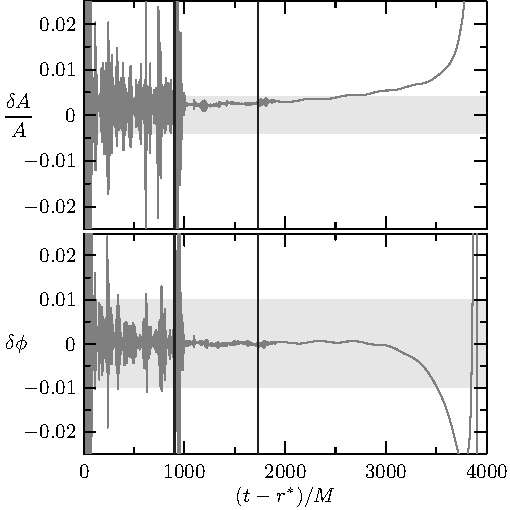
\includegraphics[width=0.55\linewidth]{figures/comparison/PlotDifferences}
  \end{center}
  \caption{Amplitude and phase differences between the numerical and
    post-Newtonian waveforms, $\Psi_4$, that are blended to create the
    hybrid waveform.  The vertical lines at $900M$ and $1730M$ denote
    the region over which matching and hybridization occur.  Note that
    the agreement is well within the numerical accuracy of the
    simulation, represented by the horizontal bands, throughout the
    matching region.  Also note that the phase difference is fairly
    flat for a significant period of time after the matching range,
    which indicates that the match is not sensitive to the particular
    range chosen for matching.}
  \label{fig:MatchingPhaseComparison}
\end{figure}%
%%%%%%%%%%%%%%%%%%%%%%%%%%%%%%%%%%%%%%%%%%%%%%%%%%%%%%%%%%%%%%%%%%%%%%
In Fig.~\ref{fig:MatchingPhaseComparison} we compare the phase of the
numerical and pN waveforms.  The quantities plotted are
\begin{eqnarray}
  \delta \phi & \equiv & \phi_{\pN} - \phi_{\NR}\ , \\
  \frac{\delta A}{A} & \equiv & \frac{A_{\pN} - A_{\NR}}{A_{\NR}}\ , 
\end{eqnarray}
shown over the interval on which both data sets exist.  The vertical
bars denote the matching region.  Note that the phase difference is
well within the accuracy of the simulation (about 0.01 radians,
represented by the horizontal band) over a range extending later than
the matching region.  Also, the difference between the two is fairly
flat, which implies that the match is not very sensitive to the region
chosen for matching.  Because of this, we expect that the phase
coherence between the early pN data and the late NR data will be
physically accurate to high precision.

The hybrid waveform is then constructed by blending the two matched
waveforms together according to
\begin{eqnarray}
  \label{eq:HybridWaveform}
  A_{\hyb}(t) &= & \tau(t)\, A_{\NR} + \left[ 1 - \tau(t) \right]\,
  A_{\pN}(t)\ , \\
  \phi_{\hyb}(t) &= & \tau(t)\, \phi_{\NR} + \left[ 1 - \tau(t)
  \right]\, \phi_{\pN}(t)\ .
\end{eqnarray}
The blending function $\tau$ is defined by

\begin{equation}
  \label{eq:BlendingFunction}
  \tau(t) = \left\{\begin{array}{ll}
      0 & \mathrm{if}\quad t<t_{1}  \\
      \frac{t-t_{1}}{t_{2}-t_{1}} & \mathrm{if}\quad t_{1} \leq t < t_{2} \\
      1 & \mathrm{if}\quad t_{2} \leq t
    \end{array} \right.
\end{equation}

The values of $t_{1}$ and $t_{2}$ are the same as those used for the
matching.  The amplitude discrepancy between the pN waveform and the
NR waveform over this interval is within numerical
uncertainty---roughly $0.4\%$.  As with the matching technique
(Eq.~(\ref{eq:MatchingChiSquared})), this method is similar to that of
Ref.~\cite{Ajith-Babak-Chen-etal:2007b}, but distinct, in that we
blend the phase and amplitude, rather than the real and imaginary
parts.  This leads to a smoothly blended waveform, shown in
Fig~\ref{fig:WaveformSnapshot}.
%%%%%%%%%%%%%%%%%%%%%%%%%%%%%%%%%%%%%%%%%%%%%%%%%%%%%%%%%%%%%%%%%%%%%%
\begin{figure}
  \begin{center}
    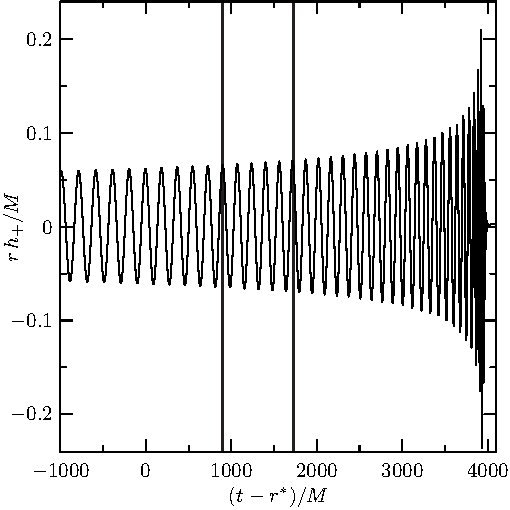
\includegraphics[width=0.55\linewidth]{figures/comparison/Waveform}
  \end{center}
  \caption{The last $t=5000\MSun$ of the hybrid waveform used in this
    analysis: the $h_{+}$ waveform seen by an observer on the positive
    $z$ axis.  The vertical lines denote the matching and
    hybridization region.  The $0$ on the time axis corresponds to the
    beginning of data from the numerical simulation.}
  \label{fig:WaveformSnapshot}
\end{figure}%
%%%%%%%%%%%%%%%%%%%%%%%%%%%%%%%%%%%%%%%%%%%%%%%%%%%%%%%%%%%%%%%%%%%%%%

Up to this point, the waveform has been $\Psi_{4}$ data.  With the
long waveform in hand, we numerically integrate twice to obtain $h$,
and set the four integration constants so that the final waveform has
zero average and first moment~\cite{Pfeiffer-Brown-etal:2007}.
Because of the very long duration of the waveforms, this gives a
reasonable result, which is only incorrect at very low
frequencies---lower than any frequency of interest to us.  We have
also checked that our results do not change when we effectively
integrate in the frequency domain by taking
\begin{equation}
  \label{eq:PsiFourIntegration}
  \tilde{h} = -\frac{\tilde{\Psi}_{4}}{4\,\pi\, f^{2}}\ ,
\end{equation}
which is the frequency-domain analog of the equation $\Psi_{4} =
\ddot{h}$.
\fi
\section{Conclusions}

In this chapter we reviewed the basic properties of gravitational
waves and methods used to model such waves from the inspiral and
merger of systems of compact binaries.  In the next chapter we discuss
the principles behind an ongoing experiment to directly observe
gravitational radiation.


% Todo:
% Discuss the Weyl tensor, if needed for NR
